
% how to compile: platex xxx.tex ; dvipdfmx xxx.dvi

\documentclass[a4paper]{jarticle}


%--余白の設定
\setlength{\topmargin}{20mm}
\addtolength{\topmargin}{-1in}
\setlength{\oddsidemargin}{20mm}
\addtolength{\oddsidemargin}{-1in}
\setlength{\evensidemargin}{15mm}
\addtolength{\evensidemargin}{-1in}
\setlength{\textwidth}{170mm}
\setlength{\textheight}{254mm}
\setlength{\headsep}{0mm}
\setlength{\headheight}{0mm}
\setlength{\topskip}{0mm}

%--ハイバーリンクを可能にするパッケージ
\usepackage[dvipdfmx,%
 bookmarks=true,%
 bookmarksnumbered=true,%
 colorlinks=true,%
 setpagesize=false,%
 pdftitle={mcat},%
 pdfauthor={BMRC},%
 pdfkeywords={TeX; dvipdfmx; hyperref; color;}]{hyperref}

\usepackage{graphicx}
\usepackage{tabularx}

\begin{document}

\setlength{\baselineskip}{4mm}

\section*{kago\_itemset.rb コマンド}
トランザクションデータから頻出アイテム集合を列挙する。
アイテム集合の他にも、飽和アイテム集合、極大アイテム集合も列挙できる。
列挙のコアアルゴリズムにはLCM(Linear time Closed itemset Miner)を用いている\cite{Uno2004,UnoWeb}。
また、アイテムの階層分類を導入することもでき、
異なる分類間の頻出アイテム集合を求めることができる。
さらに、クラス項目を指定することで、それぞれのクラスにのみ多頻度なアイテム集合である顕在パターン(emerging patterns)を列挙することもできる。

\begin{table}[htbp]
\begin{center}
\begin{tabular}{ccc}

\begin{minipage}{0.3\hsize}
\begin{center}
\caption{key型データ\label{tbl:key}}
{\small
\begin{tabular}{cc}
\hline
key&item \\
\hline
T1&C \\
T1&E \\
T2&D \\
T2&E \\
T2&F \\
:&: \\ \hline
\end{tabular} 
}
\end{center}
\end{minipage}

\begin{minipage}{0.3\hsize}
\begin{center}
\caption{tra型データ\label{tbl:tra}}
{\small
\begin{tabular}{ll}
\hline
id&item \\
\hline
T1&C E \\
T2&D E F \\
T3&A B D F \\
T4&B D F \\
T5&A B D E \\
T6&A B D E F \\
\hline
\end{tabular} 
}
\end{center}
\end{minipage}

\begin{minipage}{0.3\hsize}
\begin{center}
\caption{行列型データ\label{tbl:matrix}}
{\small
\begin{tabular}{ccccccc}
\hline
id&A&B&C&D&E&F \\
\hline
T1& & &1& &1& \\
T2& & & &1&1&1\\
T3&1&1& &1& &1\\
T4& &1& &1& &1\\
T5&1&1& &1&1& \\
T6&1&1& &1&1&1\\
\hline
\end{tabular} 
}
\end{center}
\end{minipage}

\end{tabular} 
\end{center}
\end{table} 

入力データとしては、表\ref{tbl:key},\ref{tbl:tra},\ref{tbl:matrix}で示される
ような多様なデータ型を用いることができるが、
本コマンドが直接扱うのはkey型データ(表\ref{tbl:key})のみである。
その他のデータ型は、\verb|kago_t2k.rb|および\verb|kago_m2k.rb|コマンドによって、
あらかじめkey型データに変換しておく必要がある。


\subsubsection*{頻出アイテム集合}
頻出アイテム集合とは、出現頻度(サポートと呼ぶ)が
ユーザの与えた最小サポート以上であるようなアイテム集合のことを言う。
表\ref{tbl:tra}を例にとると、最小サポートが3件とすると、
アイテム集合\{B,D,F\}はT3,T5,T6の3件に出現しているので頻出であるが
アイテム集合\{B,D,E\}はT5,T6の2件にしか出現していないので頻出ではない。
ここで最小サポート3件を満たす頻出アイテム集合は、
\{A\},
\{A,B\},
\{A,B,D\},
\{A,D\},
\{B\},
\{B,D\},
\{B,D,F\},
\{B,F\},
\{D\},
\{D,E\},
\{D,F\},
\{E\},
\{F\}
の計13件である。

頻出アイテム集合を列挙すると、時にその数は膨大なものとなる。
そこで、列挙された頻出アイテム集合から代表的なアイテム集合のみを出力する
方法として、飽和アイテム集合と極大アイテム集合の列挙がある。

\subsubsection*{飽和アイテム集合}
任意の二つの頻出アイテム集合について、
それらのアイテム集合が出現するトランザクションが同じであれば、
それら二つのアイテム集合は同じグループに属すると考える。
このようにして頻出アイテム集合をグルーピングすると、
各グループには、そのサイズが最も大きいアイテム集合がただ一つあることが分かっている。
このような頻出アイテム集合を飽和アイテム集合と呼ぶ。
例えば、\{A\},\{A,B\},\{A,D\},\{A,B,D\}は全てT3,T5,T6のトランザクションに出現するので同一グループである。
そしてこの中で最もサイズの大きい\{A,B,D\}が飽和集合ととして出力され、\{A\},\{A,B\},\{A,D\}は出力されない。
全ての飽和集合を列挙すると7パターンとなり、
飽和集合という代表的なアイテム集合を列挙することで件数を大幅に減少できている。
%ただし、データによっては、飽和集合を列挙したとしても全く列挙件数が減少しない
%ことも有りうる。

\begin{table}[htbp]
\begin{center}

\caption{飽和アイテム集合\label{tbl:close}}
{\small
\begin{tabular}{lll}
\hline
飽和集合&出現トランザクション&グループ \\
\hline
\{A,B,D\} & T3,T5,T6       & \{A\},\{A,B\},\{A,D\},\{A,B,D\} \\
\{B,D\}   & T3,T4,T5,T6    & \{B\},\{B,D\}  \\
\{B,D,F\} & T3,T4,T6       & \{B,F\},\{B,D,F\} \\
\{D\}     & T2,T3,T4,T5,T6 & \{D\} \\
\{D,E\}   & T2,T5,T6       & \{D,E\}    \\
\{D,F\}   & T2,T3,T4,T6    & \{F\},\{D,F\} \\
\{E\}     & T1,T2,T5,T6    & \{E\} \\ \hline
\end{tabular} 
}

\end{center}
\end{table} 

\subsubsection*{極大アイテム集合}
頻出アイテム集合のあるアイテム集合について、そのアイテム集合が
その他のアイテム集合に包含されていなければ、
そのアイテム集合を極大アイテム集と呼ぶ。
表\ref{tbl:tra}においては、\{A,B,D\},\{B,D,F\},\{D,E\}の3つのアイテム集合は、
他のどのアイテム集合にも包含されないので極大アイテム集合である。
その他のアイテム集合は、上記3つの極大アイテム集合のいずれかに包含されているため
極大ではない。

\subsubsection*{顕在パターン}
各トランザクションが属する「クラス」を導入し、あるクラスに特徴的なパターン(ここでは頻出アイテム集合)を列挙する。
ここで特徴的とは、あるクラスには多頻度で、他のクラスでは多頻度でないことである。
例えば、スーパーマーケットでは、男性と女性で購買されるアイテムの違いを識別したい時などに使われる。



\subsubsection*{階層分類}
アイテムの階層分類を反映させることができる。
例えば、スーパーマーケットでは「◯◯牛乳500ml」というアイテムは
「牛乳」に分類され、「牛乳」は「乳製品」に分類され、
さらに「乳製品」は食品に分類される。
このような階層分類を導入することで、「◯◯牛乳500ml」は「果物」と
購入される頻度が多いといった、階層分類の異なるアイテム間の関係を見つけることが
できるかもしれない。
ただし、現行バージョンでは、階層は1段階のみ対応している。

内部で行われる処理は至ってシンプルで、アイテムと分類の対応関係(表\ref{tbl:map})を与え、
入力データ(表\ref{tbl:org})のアイテムに応じた分類アイテムを追加(表\ref{tbl:add})、もしくは置換(表\ref{tbl:rep})した後に、
頻出アイテム集合を求める。

\begin{table}[htbp]
\begin{center}
\begin{tabular}{ccc}

\begin{minipage}{0.25\hsize}
\begin{center}
\caption{元データ\label{tbl:org}}
{\small
\begin{tabular}{ll}
\hline
id&item \\
\hline
T1&C E \\
T2&D E F \\
T3&A B D F \\
T4&B D F \\
T5&A B D E \\
T6&A B D E F \\
\hline
\end{tabular} 
}
\end{center}
\end{minipage}

\begin{minipage}{0.25\hsize}
\begin{center}
\caption{item-分類対応表\label{tbl:map}}
{\small
\begin{tabular}{cc}
\hline
item&taxonomy \\
\hline
A&X \\
B&X \\
C&Y \\
D&Z \\
E&Z \\
F&Z \\ \hline
\end{tabular} 
}
\end{center}
\end{minipage}

\begin{minipage}{0.25\hsize}
\begin{center}
\caption{分類追加後データ\label{tbl:add}}
{\small
\begin{tabular}{ll}
\hline
id&item \\
\hline
T1&C E Y Z\\
T2&D E F Z \\
T3&A B D F X Z\\
T4&B D F Y Z\\
T5&A B D E X Z\\
T6&A B D E F X Z\\
\hline
\end{tabular} 
}
\end{center}
\end{minipage}

\begin{minipage}{0.25\hsize}
\begin{center}
\caption{分類置換後データ\label{tbl:rep}}
{\small
\begin{tabular}{ll}
\hline
id&item \\
\hline
T1&Y Z\\
T2&Z \\
T3&X Z\\
T4&Y Z\\
T5&X Z\\
T6&X Z\\
\hline
\end{tabular} 
}
\end{center}
\end{minipage}


\end{tabular} 
\end{center}
\end{table} 


\subsection*{書式}
\begin{verbatim}
kago_itemset.rb i= [type=] tid= item= [class=] [s=|S=] [top=] [p=] [l=] [u=] [O=] [x=] [taxo=] [--help]
\end{verbatim}

\begin{table}[htbp]
%\begin{center}
{\small
\begin{tabular}{ll}
\verb|i=|    & key型トランザクションデータファイル名【必須】 \\
\verb|type=| & アイテム集合のタイプ(\verb|F|:頻出アイテム集合, \verb|C|:飽和アイテム集合, \verb|M|:極大アイテム集合【オプション: default=\verb|F|】\\
\verb|tid=|  & トランザクションID項目名【必須】\\
\verb|item=| & アイテム項目名【必須】 \\
\verb|s=|    & 最小サポート(確率)【選択必須:\verb|s=, S=|】\\
\verb|S=|    & 最小サポート(件数)【選択必須:\verb|s=, S=|】\\
\verb|top=|  & サポート上位件数【オプション】\\
\verb|p=|    & 事後確率【オプション:default=0.6】\\
\verb|g=|    & 増加率【オプション:デフォルトはp=の指定で動作する】\\
\verb|l=|    & 最小アイテム集合サイズ【オプション:default=1】\\
\verb|u=|    & 最大アイテム集合サイズ【オプション:default=5】\\
\verb|O=|    & 出力パス名【オプション:default=\verb|./kago_#{日付時刻}|】\\
\verb|c=|    & クラス名【オプション】 \\
\verb|class=|& クラス項目名【条件付き必須:\verb|c=|】 \\
\verb|x=|    & 階層分類データファイル名【オプション】\\
\verb|taxo=| & 分類項目名【条件付き必須:\verb|x=|】\\

\end{tabular} 
}
%\end{center}
\end{table} 


%\begin{description}
%\setlength{\itemindent}{0mm}
%\item[i=    ] key型トランザクションデータファイル名【必須】
%\item[type= ] アイテム集合のタイプ(F:頻出アイテム集合,C:飽和アイテム集合,M:極大アイテム集合【オプション: default=F】
%\item[tid=  ] トランザクションID項目名【必須】
%\item[item= ] アイテム項目名【必須】
%\item[s=    ] 最小サポート(確率)【選択必須:s=$|$S=$|$top=】
%\item[S=    ] 最小サポート(件数)【選択必須:s=$|$S=$|$top=】
%\item[top=  ] サポート上位件数【選択必須:s=$|$S=$|$top=】
%\item[l=    ] 最小アイテム集合サイズ【オプション】
%\item[u=    ] 最大アイテム集合サイズ【オプション】
%\item[O=    ] 出力パス名【オプション:default=./kago\_\#\{日付時刻\}】
%\item[x=    ] 階層分類データファイル名【オプション】
%\item[taxo= ] 分類項目名【条件付き必須:x=】
%\end{description}

%\subsection*{備考}
%本コマンドで使われている列挙のコアアルゴリズムにはLCM(Linear time Closed itemset Miner)を用いている。
%詳細は以下の文献およびWebページを参照されたい。
%\begin{itemize}
%\item  Takeaki Uno, Tatsuya Asai, Yuzo Uchida, Hiroki Arimura, "An Efficient Algorithm for Enumerating Closed Patterns in Transaction Databases", Discovery Science 2004, LNAI 3245, pp.16-31.
%\item http://research.nii.ac.jp/~uno/codes-j.htm
%\end{itemize}

\subsection*{利用例}
\subsubsection*{例1 頻出アイテム集合の列挙例}

\begin{verbatim}
------------------------------------------------
# tra1.csv
tid,item
T1,C
T1,E
T2,D
T2,E
T2,F
T3,A
T3,B
T3,D
T3,F
T4,B
T4,D
T4,F
T5,A
T5,B
T5,D
T5,E
T6,A
T6,B
T6,D
T6,E
T6,F

$ kago_itemset.rb S=3 tid=tid item=item i=tra1.csv O=result

# 列挙された頻出アイテム集合
# ./result/patterns.csv
pid,count,total,support,pattern
9,3,6,0.5,A
10,3,6,0.5,A B
11,3,6,0.5,A B D
12,3,6,0.5,A D
3,4,6,0.6666666667,B
4,4,6,0.6666666667,B D
8,3,6,0.5,B D F
7,3,6,0.5,B F
0,5,6,0.8333333333,D
2,3,6,0.5,D E
6,4,6,0.6666666667,D F
1,4,6,0.6666666667,E
5,4,6,0.6666666667,F

# 上記項目の説明
# pid: パターン(アイテム集合)ID
# count: 出現件数(トランザクション数)
# total: 全トランザクション数
# support: 出現確率(=count/total)
# pattern: アイテム集合(スペース区切り)

# 各トランザクションにどのpattern(pid)が出現するかの対応表
# ./result/tid_pats.csv
tid,pid
T1,1
T2,0
T2,5
T2,2
 :
# 上記項目の説明
# tid: トランザクションID(入力データのtid項目に対応)
# pid: パターンID(pattern.csvのpidに対応)
------------------------------------------------
\end{verbatim}

\subsubsection*{例2 アイテム集合のサイズに制限を加えた例}

\begin{verbatim}
------------------------------------------------
$ kago_itemset.rb S=3 l=3 u=3 tid=tid item=item i=tra1.csv O=result

# ./result/patterns.csv
tid,count,total,support,pattern
1,3,6,0.5,A B D
0,3,6,0.5,B D F
------------------------------------------------
\end{verbatim}

\subsubsection*{例3 飽和集合の列挙例}

\begin{verbatim}
------------------------------------------------
$ kago_itemset.rb S=3 type=C tid=tid item=item i=tra1.csv O=result

# ./result/patterns.csv
pid,count,total,support,pattern
6,3,6,0.5,A B D
3,4,6,0.6666666667,B D
5,3,6,0.5,B D F
0,5,6,0.8333333333,D
2,3,6,0.5,D E
4,4,6,0.6666666667,D F
1,4,6,0.6666666667,E
------------------------------------------------
\end{verbatim}

\subsubsection*{例4 極大集合の列挙例}

\begin{verbatim}
------------------------------------------------
$ kago_itemset.rb S=3 type=M tid=tid item=item i=tra1.csv O=result

# ./result/patterns.csv
pid,count,total,support,pattern
2,3,6,0.5,A B D
1,3,6,0.5,B D F
0,3,6,0.5,D E
------------------------------------------------
\end{verbatim}

\subsubsection*{例5 階層分類を使った例}

\begin{verbatim}
------------------------------------------------
# taxo.csv
# item,taxonomy
A,X
B,X
C,Y
D,Z
E,Z
F,Z

$ kago_itemset.rb S=4 tid=tid item=item i=tra1.csv x=taxo.csv taxo=taxonomy O=result

# ./result/patterns.csv
pid,pattern,count,total,support
0,Z,6,6,1
1,D Z,5,6,0.8333333333
2,E Z,4,6,0.6666666667
3,F Z D,4,6,0.6666666667
4,X Z D B,4,6,0.6666666667
------------------------------------------------
\end{verbatim}

\subsubsection*{例6 オリジナルアイテムを階層分類で置換する例}
\begin{verbatim}
------------------------------------------------
$ kago_itemset.rb S=4 tid=tid item=item i=tra1.csv x=taxo.csv taxo=taxonomy O=result -replaceTaxo

# ./result/patterns.csv
pid,count,total,support,pattern
1,4,6,0.6666666667,X Z
0,6,6,1,Z
------------------------------------------------
\end{verbatim}

\subsubsection*{例7 顕在パターンの列挙例}
\begin{verbatim}
------------------------------------------------
# class.csv
tid,class
T1,cls1
T2,cls1
T3,cls1
T4,cls1
T5,cls2
T6,cls2

$ kago_itemset.rb S=3 tid=tid item=item i=tra1.csv c=class.csv class=class p=0.6 O=result

# ./result/patterns.csv
class,pid,pattern,pos,neg,posTotal,negTotal,total,support,growthRate,postProb
cls2,18,D A E,2,0,2,4,6,1,inf,1
cls2,15,D B E,2,0,2,4,6,1,inf,1
              :
cls1,6,B F,2,1,4,2,6,0.5,1,0.5
cls1,0,D,3,2,4,2,6,0.75,0.75,0.4285714286
------------------------------------------------
\end{verbatim}

\subsection*{関連コマンド}

\hyperlink{kago\_m2k.pdf}{kago\_m2k} : matrix型データの変換

\subsection*{資料1: パラメータgr=,post=,-unifについて}
クラス集合$C=\{c_1,c_2,\cdots,c_m\}$があり、各トランザクションは、いずれか一つのクラスに属しているものとする。
ここで我々が興味のある顕在パターンとは、ある対象クラスに頻出し、その他のクラスに頻出すしないようなアイテム集合である。
例えば、対象クラス$c_1$に頻出し、その他のクラス$c_2,c_3,\cdots,c_m$には頻出しないようなアイテム集合である。
以降、対象クラスを$c_t$、その他のクラスを$c_o$で表すものとする。

本コマンドでは顕在パターンを以下の3種類の方法により定義できる。
\begin{enumerate}
\item 増加率(クラス間の出現確率の比)の閾値を指定
\item 事後確率の閾値を指定(事前確率はデータ上の分布から推定)
\item 事後確率の閾値を指定(事前確率は各クラス一様)
\end{enumerate}

\subsubsection*{1.増加率}

対象クラス$c_t$におけるアイテム集合$I$の増加率$GR_t(I)$は式(\ref{gr})で表され、
対象クラスとその他クラスにおけるアイテム集合の出現確率の比として定義される。
そして、顕在パターンとは、ユーザが与えた最小増加率$\gamma$以上の増加率を持つようなアイテム集合のことである。
$\gamma$は、パラメータ\verb|gr=|によって指定する。

\begin{equation}
GR_t(I)=\frac{\Pr(I|c_t)}{\Pr(I|c_o)} \ge \gamma \label{gr}
\end{equation}
%\begin{equation}
%GR_t(I) \ge \gamma \label{minGR}
%\end{equation}

\subsubsection*{2.事後確率}

%\item 事前確率は各クラス一様であると仮定した場合の、アイテム集合が観測後の対象クラスである事後確率がある閾値以上のアイテム集合
%\item アイテム集合が観測されたとき、対象クラスである事後確率がある閾値以上のアイテム集合

クラス未知のあるトランザクションについて、アイテム集合$I$を観測したとき、
そのトランザクションがクラス$c_t$に属する確率は、ベイズの定理より式(\ref{bayes})で表される。
この式は、クラス$c_t$の事前確率$\Pr(c_t)$がアイテム集合$I$を観測することで
事後確率$\Pr(c_t|I)$に更新されたことを意味する。
事前確率$\Pr(c_t)$は、与えられたデータにおけるクラス分布に基づいて推定する。
%すなわち、全トランザクション数に対するクラス$c_t$に属するトランザクションの割合である。
ここで、顕在パターンとは、ユーザが与えた最小事後確率$\pi$以上の事後確率を持つようなアイテム集合のことである。
$\pi$は、パラメータ\verb|post=|によって指定する。

\begin{equation}
\Pr(c_t|I)=\frac{\Pr(I|c_t)\Pr(c_t)}{\Pr(I|c_t)\Pr(c_t)+\Pr(I|c_o)\Pr(c_o)} \ge \pi \label{bayes}
%\Pr(c_t|I)=\frac{\Pr(I|c_t)}{\Pr(I)}\Pr(c_t) \ge \pi \label{bayes}
\end{equation}

\subsubsection*{3.事後確率(事前確率一様)}
全てのクラスの事前確率は一様であると仮定して上記の事後確率を計算する。
$\Pr(c_t)=\frac{1}{m}$,$\Pr(c_o)=\frac{m-1}{m}$を式(\ref{bayes})に代入すると式(\ref{bayes2})が得られる。
そして、顕在パターンとは、事前確率が一様であると仮定のもと、
ユーザが与えた最小事後確率$\pi_u$以上の事後確率を持つようなアイテム集合のことである。
$\pi_u$は、パラメータ\verb|post=|によって指定し、かつ\verb|-unif|オプションを指定する。

\begin{equation}
%\Pr(c_t|I)=\frac{\Pr(I|c_t)\Pr(c_t)}{\Pr(I|c_t)\Pr(c_t)+\Pr(I|c_o)\Pr(c_o)} \label{bayes}
\Pr(c_t|I)=\frac{\Pr(I|c_t)}{\Pr(I|c_t)+(m-1)\Pr(I|c_o)} \ge \pi_{u} \label{bayes2}
\end{equation}

\subsubsection*{$GR_t(I)$と$Pr(c_t|I)$の関係}
式(\ref{gr})と式(\ref{bayes})より、$GR_t(I)$と$Pr(c_t|I)$の関係は式(\ref{relgrpost})で表される。
最小事後確率$\pi$を指定して顕在パターンを列挙する場合、
内部的には式(\ref{relgrpost})に従い、$\pi$を最小増加率$\gamma$に変換して実行している。

\begin{equation}
%\Pr(c_t|I)=\frac{\Pr(I|c_t)\Pr(c_t)}{\Pr(I|c_t)\Pr(c_t)+\Pr(I|c_o)\Pr(c_o)} \label{bayes}
GR_t(I)=\frac{\Pr(c_o)}{\Pr(c_t)}\cdot \frac{\Pr(c_t|I)}{1-\Pr(c_t|I)} \label{relgrpost}
\end{equation}

\subsection*{資料2: LCMによる顕在パターン列挙について}

正例,負例のデータ集合をそれぞれ$D_t,D_o$とし,それらのサイズは$|D_t|=W |D_o|$の関係にあるとする.
いま,あるアイテム集合$I$(以下ではパターン$I$と呼ぶ)について,$D_t$における増加率$GR_t(I)$および出現ゲイン$Gain_t(I)$をそれぞれ式(\ref{gp}),(\ref{gain})の通り定義する.

\begin{equation}
GR_t(I)=\frac{sup(I,D_t)/|D_t|}{sup(I,D_o)/|D_o|}=W\frac{sup(I,D_t)}{sup(I,D_o)} \label{gp}
\end{equation}

\begin{equation}
%Gain_p(I)=\omega sup(I,D_t) /|D_t| - sup(I,D_o) /|D_o| \label{gain}
Gain_p(I)=\omega sup(I,D_t) - sup(I,D_o) \label{gain}
\end{equation}

ここで,$sup(I,D_t),sup(I,D_o)$はパターン$I$の$D_t,D_o$における出現件数で,
$\omega$は正例の出現数に与えるウェイトを表している.
パターン$I$について,$GR_t(I)$がユーザによって与えられた最小増加率
$\gamma$以上の場合,そのパターンを顕在パターンと呼び,
$Gain_p(I)$がユーザによって与えられた最小サポート$\sigma$以上の場合,
そのパターンをコントラストパターンと呼ぶことにする.
顕在パターンおよびコントラストパターンを正例,負例における
出現数の関係で示すと式(\ref{sup1}),(\ref{sup2})の通りとなる.

\begin{equation}
sup(I,D_o)\le \frac{W}{\gamma} sup(I,D_t) \label{sup1}
\end{equation}

\begin{equation}
sup(I,D_o)\le \omega sup(I,D_t) - \sigma \label{sup2}
\end{equation}

そして、負例における出現数$sup(I,D_o)$を$y$軸に,正例における出現数$sup(I,D_t)$を$x$軸としたとき,
顕在パターンは図\ref{fig:ep}の網かけで示された領域に属するパターンであり,
コントラストパターンは図\ref{fig:cp}の網かけで示された領域に属するパターンである.

\begin{figure}[htbp]
\begin{center}
\begin{tabular}{c}

\begin{minipage}{0.3\hsize}
\begin{center}
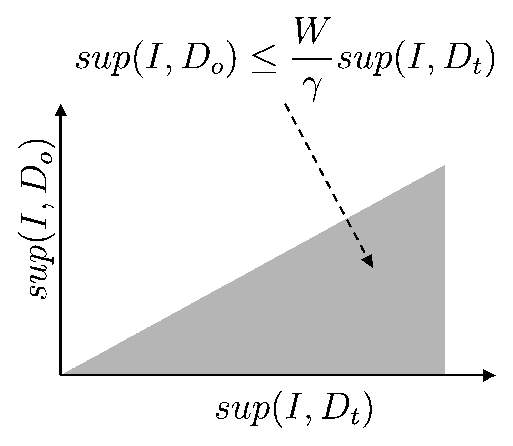
\includegraphics[scale=0.5]{./ep.eps}
\caption{顕在パターン\label{fig:ep}}
\end{center}
\end{minipage}

\begin{minipage}{0.3\hsize}
\begin{center}
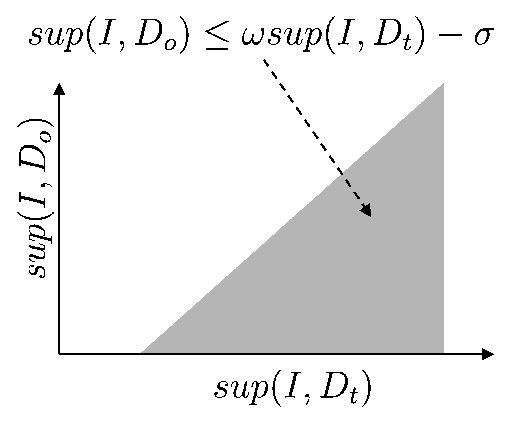
\includegraphics[scale=0.5]{./cp.eps}
\caption{コントラストパターン\label{fig:cp}}
\end{center}
\end{minipage}

\begin{minipage}{0.3\hsize}
\begin{center}
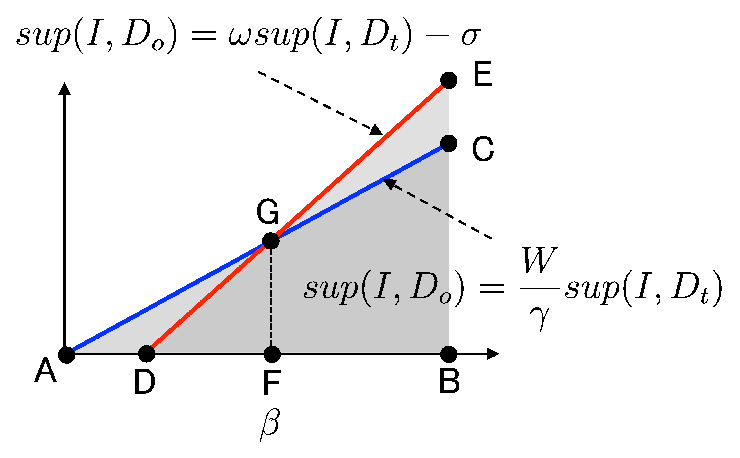
\includegraphics[scale=0.5]{./epcp.eps}
\caption{2つのパターンの関係\label{fig:epcp}}
\end{center}
\end{minipage}


\end{tabular} 
\end{center}
\end{figure} 

LCMでは,ユーザがパラメータ$\omega, \sigma$を与えることで
コントラストパターンを高速に列挙することができる.
コントラストパターンの列挙においては、$sup(I,D_t)$が大きくなればなるほど、
$sup(I,D_o)$との差が相対的に小さいパターンが列挙されることもあり、
そのようなパターンはクラス$c_t$に特徴的なパターンとは言えなくなる。
この欠点を回避するために、本コマンドでは顕在パターンの列挙を採用している。

ここで問題となるのは、コントラストパターンを列挙するLCMを使って、
いかに顕在パターンを列挙するかであり、以下に本コマンドで採用している方法を示す。

図\ref{fig:epcp}は、図\ref{fig:ep}と図\ref{fig:cp}を重ねた図である。
ここでは顕在パターンの領域ABCを全て列挙するのではなく、
$sup(I,D_t)\ge\beta$($\beta$は本コマンドS=で指定するパラメータ)を満たす領域GFCBに属する顕在パターンの列挙を考える。
LCMによって列挙されるパターンは、$\triangle{DEB}$に属するパターンであるが、
直線DEは、$\sigma$と$\omega$を定めることによって決まる。
まず$\sigma$は、直線ACと直線DEの交点Gの$x$座標が、ちょうど$\beta$になるように
設定する(式(\ref{sigma_beta}):$\omega$の決め方は後述)。
そうすることで、LCMが列挙した全パターンから、
$\triangle{DFG}$および$\triangle{EGC}$に属する
パターンを削除すれば、目的とする顕在パターンを列挙することが可能となる。

\begin{equation}
\sigma=\beta (\omega-\frac{W}{\gamma})  \label{sigma_beta}
\end{equation}



次に$\omega$であるが、これは直線DEの傾きを決めることに対応する。
一般的に$\triangle{EGC}$に属するパターンより、$\triangle{DGF}$に属するパターンの方が遥かに多いので、
$\omega$をできる限り大きくする方が効率的である。

しかしながら、$\omega$はトランザクションの重みであり、計算機上で件数をカウント
する変数の型の最大値に制約される。
その最大値を$maxInt$とすると、$\omega sup(I,D_t)\le maxInt$の制約を
満たしていなければならない。
$sup(I,D_t)$は$|D_p|$を超えることはないので、$\omega$を式(\ref{omega})のとおり
指定することで、$\triangle{DFG}$の列挙数を最小化できる。

\begin{equation}
\omega=\frac{maxInt}{|D_t|} \label{omega}
\end{equation}

\begin{thebibliography}{9}
\bibitem{Uno2004}
Takeaki Uno, Tatsuya Asai, Yuzo Uchida, Hiroki Arimura, "An Efficient Algorithm for Enumerating Closed Patterns in Transaction Databases", {\it Discovery Science 2004}, LNAI 3245, pp.16-31.
\bibitem{UnoWeb}
http://research.nii.ac.jp/~uno/codes-j.htm
\end{thebibliography}

\end{document}

